% Requires: \usepackage{subcaption}, \usepackage{graphicx}
% Place in appendix. All strip PDFs live in figures/.

\begin{figure}[p]
  \centering

  % (a) Both correct — swap present (CRAFT, detect)
  \begin{subfigure}[b]{\linewidth}
    \centering
    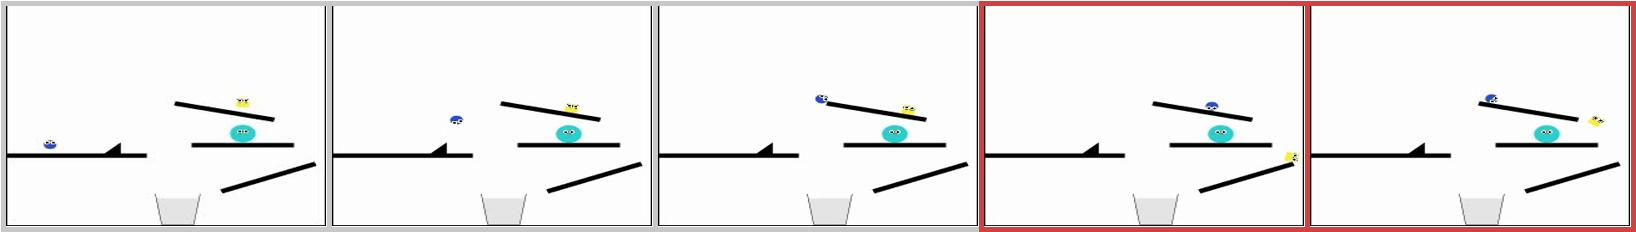
\includegraphics[width=\linewidth]{figures/both_correct_craft_scene_5_002227_strip}
    \label{fig:quadrant:both-correct-swap}
  \end{subfigure}

  \smallskip

  % (b) Both correct — no swap (MTL-AQA, detect)
  % 4-frame strip: scaled to same thumbnail size as the 5-frame strips
  \begin{subfigure}[b]{\linewidth}
    \centering
    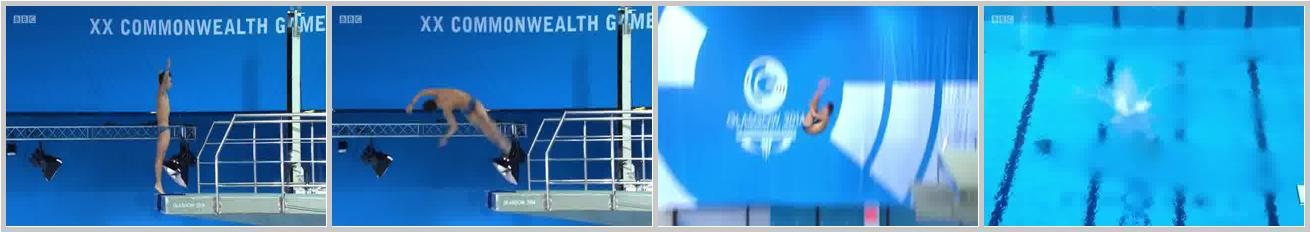
\includegraphics[width=0.8\linewidth]{figures/both_correct_mtl-aqa_scene_26_117_strip}
    \label{fig:quadrant:both-correct-noswap}
  \end{subfigure}

  \smallskip

  % (c) LLMs correct, human wrong — no swap (Drive-LM, detect)
  \begin{subfigure}[b]{\linewidth}
    \centering
    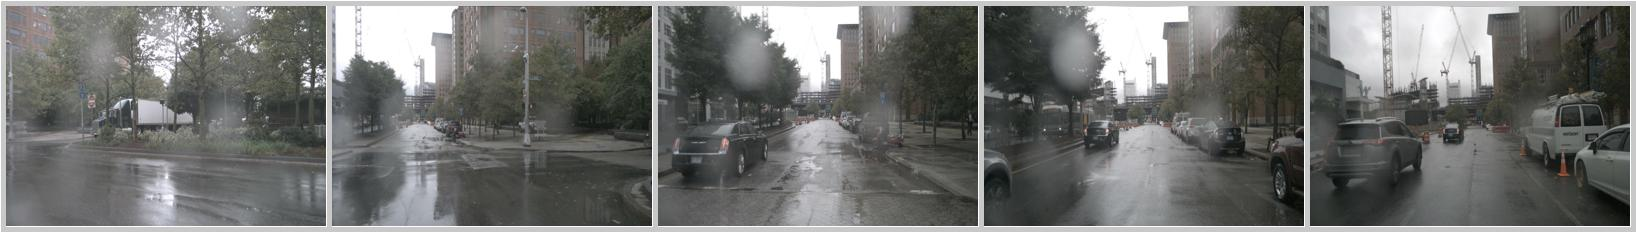
\includegraphics[width=\linewidth]{figures/llm_correct_drive-lm_scene_429_strip}
    \label{fig:quadrant:llm-correct}
  \end{subfigure}

  \smallskip

  % (d) Both wrong — swap at positions 3–4 (MTL-AQA, localize)
  \begin{subfigure}[b]{\linewidth}
    \centering
    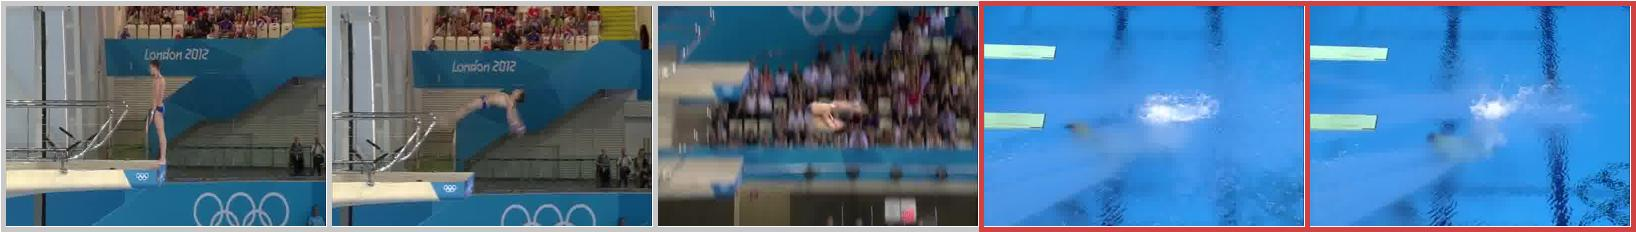
\includegraphics[width=\linewidth]{figures/both_wrong_mtl-aqa_localize_scene_02_77_strip}
    \label{fig:quadrant:both-wrong}
  \end{subfigure}

  \caption{%
    Qualitative examples illustrating the four agreement quadrants between
    human annotators and LLMs on the temporal misalignment tasks.
    Red borders mark the swapped frame pair.
    %
    \textbf{(a)}~\textit{Both correct — swap present} (CRAFT, detect):
    the pair at positions~3--4 is out of order; human and all five models
    correctly identify the swap.
    %
    \textbf{(b)}~\textit{Both correct — no swap} (MTL-AQA, detect):
    the sequence is unmodified; human and all models correctly report no anomaly.
    %
    \textbf{(c)}~\textit{LLMs correct, human wrong} (Drive-LM, detect):
    the sequence is unmodified, but the human incorrectly reports a swap,
    likely misled by rainy conditions and a camera turn between frames;
    all five models answer correctly.
    %
    \textbf{(d)}~\textit{Both wrong} (MTL-AQA, localize):
    the swap at positions~3--4 (two nearly identical underwater frames)
    is missed by both the human annotator and all five models,
    who instead point to earlier positions in the sequence.
  }
  \label{fig:quadrant-examples}
\end{figure}
